\documentclass[journal,12pt,twocolumn]{IEEEtran}

\usepackage{setspace}
\usepackage{gensymb}
\singlespacing
\usepackage[cmex10]{amsmath}

\usepackage{amsthm}

\usepackage{mathrsfs}
\usepackage{txfonts}
\usepackage{stfloats}
\usepackage{bm}
\usepackage{cite}
\usepackage{cases}
\usepackage{subfig}

\usepackage{longtable}
\usepackage{multirow}

\usepackage{enumitem}
\usepackage{mathtools}
\usepackage{steinmetz}
\usepackage{tikz}
\usepackage{circuitikz}
\usepackage{verbatim}
\usepackage{tfrupee}
\usepackage[breaklinks=true]{hyperref}
\usepackage{graphicx}
\usepackage{tkz-euclide}

\usetikzlibrary{calc,math}
\usepackage{listings}
    \usepackage{color}                                            %%
    \usepackage{array}                                            %%
    \usepackage{longtable}                                        %%
    \usepackage{calc}                                             %%
    \usepackage{multirow}                                         %%
    \usepackage{hhline}                                           %%
    \usepackage{ifthen}                                           %%
    \usepackage{lscape}     
\usepackage{multicol}
\usepackage{chngcntr}

\DeclareMathOperator*{\Res}{Res}

\renewcommand\thesection{\arabic{section}}
\renewcommand\thesubsection{\thesection.\arabic{subsection}}
\renewcommand\thesubsubsection{\thesubsection.\arabic{subsubsection}}

\renewcommand\thesectiondis{\arabic{section}}
\renewcommand\thesubsectiondis{\thesectiondis.\arabic{subsection}}
\renewcommand\thesubsubsectiondis{\thesubsectiondis.\arabic{subsubsection}}


\hyphenation{op-tical net-works semi-conduc-tor}
\def\inputGnumericTable{}                                 %%

\lstset{
%language=C,
frame=single, 
breaklines=true,
columns=fullflexible
}
\begin{document}


\newtheorem{theorem}{Theorem}[section]
\newtheorem{problem}{Problem}
\newtheorem{proposition}{Proposition}[section]
\newtheorem{lemma}{Lemma}[section]
\newtheorem{corollary}[theorem]{Corollary}
\newtheorem{example}{Example}[section]
\newtheorem{definition}[problem]{Definition}

\newcommand{\BEQA}{\begin{eqnarray}}
\newcommand{\EEQA}{\end{eqnarray}}
\newcommand{\define}{\stackrel{\triangle}{=}}
\bibliographystyle{IEEEtran}
\raggedbottom
\setlength{\parindent}{0pt}
\providecommand{\mbf}{\mathbf}
\providecommand{\pr}[1]{\ensuremath{\Pr\left(#1\right)}}
\providecommand{\qfunc}[1]{\ensuremath{Q\left(#1\right)}}
\providecommand{\sbrak}[1]{\ensuremath{{}\left[#1\right]}}
\providecommand{\lsbrak}[1]{\ensuremath{{}\left[#1\right.}}
\providecommand{\rsbrak}[1]{\ensuremath{{}\left.#1\right]}}
\providecommand{\brak}[1]{\ensuremath{\left(#1\right)}}
\providecommand{\lbrak}[1]{\ensuremath{\left(#1\right.}}
\providecommand{\rbrak}[1]{\ensuremath{\left.#1\right)}}
\providecommand{\cbrak}[1]{\ensuremath{\left\{#1\right\}}}
\providecommand{\lcbrak}[1]{\ensuremath{\left\{#1\right.}}
\providecommand{\rcbrak}[1]{\ensuremath{\left.#1\right\}}}
\theoremstyle{remark}
\newtheorem{rem}{Remark}
\newcommand{\sgn}{\mathop{\mathrm{sgn}}}
\providecommand{\abs}[1]{\left\vert#1\right\vert}
\providecommand{\res}[1]{\Res\displaylimits_{#1}} 
\providecommand{\norm}[1]{\left\lVert#1\right\rVert}
%\providecommand{\norm}[1]{\lVert#1\rVert}
\providecommand{\mtx}[1]{\mathbf{#1}}
\providecommand{\mean}[1]{E\left[ #1 \right]}
\providecommand{\fourier}{\overset{\mathcal{F}}{ \rightleftharpoons}}
%\providecommand{\hilbert}{\overset{\mathcal{H}}{ \rightleftharpoons}}
\providecommand{\system}{\overset{\mathcal{H}}{ \longleftrightarrow}}
	%\newcommand{\solution}[2]{\textbf{Solution:}{#1}}
\newcommand{\solution}{\noindent \textbf{Solution: }}
\newcommand{\cosec}{\,\text{cosec}\,}
\providecommand{\dec}[2]{\ensuremath{\overset{#1}{\underset{#2}{\gtrless}}}}
\newcommand{\myvec}[1]{\ensuremath{\begin{pmatrix}#1\end{pmatrix}}}
\newcommand{\mydet}[1]{\ensuremath{\begin{vmatrix}#1\end{vmatrix}}}
\numberwithin{equation}{subsection}

\makeatletter
\@addtoreset{figure}{problem}
\makeatother
\let\StandardTheFigure\thefigure
\let\vec\mathbf

\renewcommand{\thefigure}{\theproblem}

\def\putbox#1#2#3{\makebox[0in][l]{\makebox[#1][l]{}\raisebox{\baselineskip}[0in][0in]{\raisebox{#2}[0in][0in]{#3}}}}
     \def\rightbox#1{\makebox[0in][r]{#1}}
     \def\centbox#1{\makebox[0in]{#1}}
     \def\topbox#1{\raisebox{-\baselineskip}[0in][0in]{#1}}
     \def\midbox#1{\raisebox{-0.5\baselineskip}[0in][0in]{#1}}
\vspace{3cm}
\title{Assignment 1}
\author{KRATI ARELA - EE18BTECH11050}
\maketitle
\newpage
\renewcommand{\thefigure}{\theenumi}
\renewcommand{\thetable}{\theenumi}



Download all python codes from 
\begin{lstlisting}
https://github.com/Krati012/EE3025/tree/main/Assignment1/codes
\end{lstlisting}
and latex-tikz codes from 
\begin{lstlisting}
https://github.com/Krati012/EE3025/tree/main/Assignment1
\end{lstlisting}
%%%%%%
\section{Digital Filter}
\begin{enumerate}[label=\thesection.\arabic*
,ref=\thesection.\theenumi]
\item
\label{prob:inp}
Download the sound file from  
\begin{lstlisting}
wget https://raw.githubusercontent.com/gadepall/ 
EE1310/master/filter/codes/Sound_Noise.wav
\end{lstlisting}

\item
\label{prob:out}
Write the python code for removal of out of band noise and execute the code.
\\
\solution
\lstinputlisting{./codes/remove_noise.py}
\end{enumerate}
%%%%%%%
\section{Difference equation}

\begin{enumerate}[label=\thesection.\arabic*,ref=\thesection.\theenumi]
\item
\label{prob:diffEq}
Write the difference equation of the above Digital filter obtained in problem \ref{prob:out}.
\\
\solution
\begin{equation}
\label{eq:eqn1}
 \sum _{m=0}^{M}a\brak{m}y\brak{n-m}=\sum _{k=0}^{N}b\brak{k}x\brak{n-k}
\end{equation}
\begin{equation}
\label{eq:eqn2}
\begin{split}
y(n) - 2.52y(n-1) + 2.56y(n-2) - 1.206y(n-3)
\\
+ 0.22013y(n-4) = 0.00345x(n) + 0.0138x(n-1)
\\
+ 0.020725x(n-2) + 0.0138x(n-3) + 0.00345x(n-4)
\end{split}
\end{equation}

\item
\label{prob:plot_x_y}
Sketch x(n) and y(n).
\\
\solution
The following code yields Fig. \ref{fig:x_y}
\begin{lstlisting}
codes/x_y.py
\end{lstlisting}
The filtered sound signal obtained through difference equation is found in
\begin{lstlisting}
codes/Sound_diffEq.wav
\end{lstlisting}
\begin{figure}[!ht]
\begin{center}
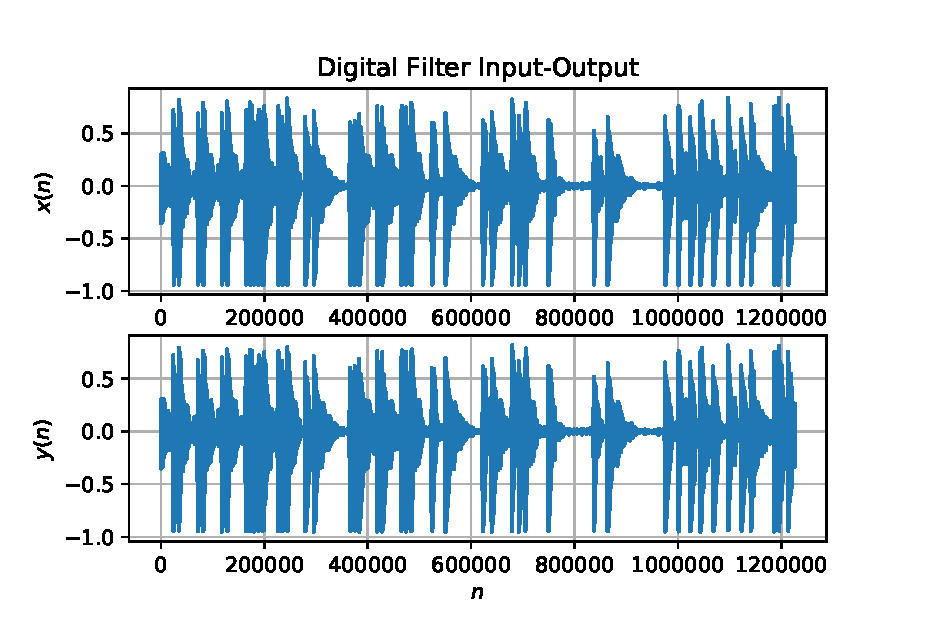
\includegraphics[width=\columnwidth]{./figs/x_y}
\end{center}
\captionof{figure}{}
\label{fig:x_y}	
\end{figure}
\end{enumerate}
%%%%%%
\section{Z-transform}

\begin{enumerate}[label=\thesection.\arabic*,ref=\thesection.\theenumi]

\item
\label{prob:Z_transf}
\begin{equation}
\label{eq:z_trans}
X(z)={\mathcal {Z}}\{x(n)\}=\sum _{n=-\infty }^{\infty }x(n)z^{-n}
\end{equation}
Show that
\begin{equation}
\label{eq:shift1}
{\mathcal {Z}}\{x(n-1)\} = z^{-1}X(z)
\end{equation}
and find
\begin{equation}
	{\mathcal {Z}}\{x(n-k)\} 
\end{equation}
\\
\solution From \eqref{eq:z_trans},
\begin{align}
{\mathcal {Z}}\{x(n-k)\} &=\sum _{n=-\infty }^{\infty }x(n-1)z^{-n}
\\
&=\sum _{n=-\infty }^{\infty }x(n)z^{-n-1} = z^{-1}\sum _{n=-\infty }^{\infty }x(n)z^{-n}
\end{align}
resulting in \eqref{eq:shift1}. Similarly, it can be shown that
\begin{equation}
\label{eq:z_trans_shift}
	{\mathcal {Z}}\{x(n-k)\} = z^{-k}X(z)
\end{equation}

\item Find
\begin{equation}
H(z) = \frac{Y(z)}{X(z)}
\end{equation}
from  \eqref{eq:eqn2} assuming that the $Z$-transform is a linear operation.
\\
\solution  Applying \eqref{eq:z_trans_shift} in \eqref{eq:eqn2} we get,
\begin{equation}
\begin{split}
H(z) = \frac{Y(z)}{X(z)}                
\\
=\frac{b[0]+b[1]z^{-1}+b[2]z^{-2}+b[3]z^{-3}+b[4]z^{-4}}{a[0]+a[1]z^{-1}+a[2]z^{-2}+a[3]z^{-3}+a[4]z^{-4}}
\label{eq:freq_resp}
\end{split}
\end{equation}

\item 
Let
\begin{equation}
H\brak{e^{\j w}} = H\brak{z = e^{\j w}}.
\end{equation}
Plot $\abs{H\brak{e^{\j w}}}$.
\\
\solution
The following code plots Fig. \ref{fig:H(jw)}.
\begin{lstlisting}
codes/dtft.py
\end{lstlisting}
\begin{figure}[!ht]
\centering
\includegraphics[width=\columnwidth]{./figs/dtft}
\caption{$\abs{H\brak{e^{\j w}}}$}
\label{fig:H(jw)}
\end{figure}
\end{enumerate}
%%%%%%%
\section{Impulse Response}
\begin{enumerate}[label=\thesection.\arabic*,ref=\thesection.\theenumi]
\item
From the difference equation eq. \ref{eq:eqn2}. Sketch h(n). 
\label{prob:hn}
\\
\solution
We know that when $x(n) = \delta(n)$ (input is impulse),  we get the Impulse response h(n) of the system as output.

From eq.\ref{eq:eqn1}, 

Substitute $x(n-k) = \delta(n-k)$, 

$y(n-k)$ becomes $h(n-k)$ for all k=0,1,2,3,4.

Now, the following code plots Fig. \ref{fig:hn}
\begin{lstlisting}
codes/hn.py
\end{lstlisting}
\begin{figure}[!ht]
\centering
\includegraphics[width=\columnwidth]{./figs/hn}
\caption{$h(n)$}
\label{fig:hn}
\end{figure}

\item Is the system defined in eq. \ref{eq:eqn2} for impulse response obtained above stable?
\\
\solution
The system is defined by the eq. \ref{eq:eqn2}
For a system to be stable, output should be bounded for every bounded input. This is known as BIBO stability.

Since the audio input x(n) is bounded, let $B_x$ be some finite value, we have
\begin{align}
    \abs{x(n)} < B_x < \infty
\end{align}
From convolution property,
\begin{equation}
    \abs{y(n)} = \abs{\sum_{-\infty}^{\infty}h(k)x(n-k)}
\end{equation}
\begin{equation}
    \abs{y(n)} \leq \sum_{-\infty}^{\infty}\abs{h(k)}\abs{x(n-k)}\\
\end{equation}
Let $B_{x}$ be the maximum value x(n-k) can take, then
\begin{equation}
\abs{y(n)} \leq B_{x}\sum_{-\infty}^{\infty} \abs{h(k)}
\end{equation}
If
\begin{equation}
\sum_{-\infty}^{\infty} \abs{h(k)} < \infty
\end{equation}
Then
\begin{equation}
\abs{y(n)} \leq B_{y} < \infty
\end{equation}

Therefore we can say that y(n) is bounded if x(n) and h(n) are bounded.

Since the audio input is bounded, the system is said to be stable if h(n) is also bounded.
\begin{equation}
\sum_{n=-\infty}^{\infty} \abs{h(n)}<\infty
\end{equation}
The above equation can be re-written as,
\begin{equation}
\sum_{n=-\infty}^{\infty} \abs{h(n)} \abs{z^{-n}}_{\abs{z}=1}<\infty
\end{equation}
\begin{equation}
\sum_{n=-\infty}^{\infty} \abs{h(n)z^{-n}}_{\abs{z}=1}<\infty
\end{equation}
From Triangle inequality,
\begin{equation}
\sum_{n=-\infty}^{\infty}\abs{h(n)z^{-n}}_{\abs{z}=1}<\abs{\sum_{n=-\infty}^{\infty}h(n)z^{-n}}_{\abs{z}=1} \\
%\abs{\sum_{-\infty}^{\infty} h(n)z^{-n}}_{\abs{z}=1}<\infty
\end{equation}
\begin{equation}
\implies \abs{H(n)}_{\abs{z}=1} < \infty
\end{equation}
Therefore, the Region of Convergence (ROC) should include the unit circle for the system to be stable.

Since, h(n) is right sided the ROC is outside the outer most pole. From the equation \eqref{eq:freq_resp}

Poles of the given transfer equation is:
\begin{equation}
\begin{split}
z(approx) = 0.694 \pm 0.41i,
\\
 0.566 \pm 0.134i
\end{split}  
\end{equation}
From the above poles, we can see that that the ROC of the system is $\abs{z}>\sqrt{0.694^{2}+0.41^{2}}$.
$\implies \abs{z} > 0.806$
\\
\begin{figure}[!ht]
\centering
\includegraphics[width=\columnwidth]{./figs/roc}
\caption{$H(z)$ in $z$-plane}
\label{fig:xnhnfft}
\end{figure}

The code for plotting H(z) in z-plane is:
\begin{lstlisting}
codes/roc.py
\end{lstlisting}

From the figure we can observe that ROC of the system includes unit circle $\abs{z}=1$.
Which implies that the given IIR filter is stable, because h(n) is absolutely summable.
\\
\textbf{Verification}:

Given input audio signal x(n) which is bounded, and system difference equation \ref{eq:eqn2}

From python code we can get that the maximum value of x(n) is 0.839 and minimum value is -0.9417.

Similarly we can also get that the maximum value of y(n) is 0.82225 and minimum value is -0.95376 and it tends to zero as n tends to infinity.

We can say that the bounded input x(n) gives bounded output
y(n). Therefore we can say that the system is BIBO stable.

\item Using h(n) obtained in \ref{prob:hn} compute filtered output using the below equation of convolution
%
\begin{equation} 
\label{eq:convolution}
y(n) = x(n)*h(n) = \sum_{n=-\infty}^{\infty}x(k)h(n-k)
\end{equation}
\solution The following code plots Fig. \ref{fig:ynconv}
%
\begin{lstlisting}
codes/ynconv.py
\end{lstlisting}
\begin{figure}[!ht]
\centering
\includegraphics[width=\columnwidth]{./figs/ynconv}
\caption{$y(n)$ from the definition of convolution}
\label{fig:ynconv}
\end{figure}
The filtered sound signal through convolution from this method is found in
\begin{lstlisting}
codes/Sound_conv.wav
\end{lstlisting}
We can observe that the output obtained is same as y(n) obtained in Fig. \ref{fig:x_y}

\end{enumerate}

\section{DFT and FFT}
\begin{enumerate}[label=\thesection.\arabic*
,ref=\thesection.\theenumi]
\item Compute
\begin{align}
        X(k) \triangleq \sum_{n=0}^{N-1} x(n) e^{-j 2 \pi k n / N}, \quad k=0,1, \ldots, N-1
\end{align}
and $H(k)$ using h(n).
\\
\solution
For this given IIR system with audio sample as x(n) and h(n) as impulse response h(n) obtained in \ref{prob:hn} 

DFT of a Input Signal $x(n)$ is 
\begin{align}
    X(k) \triangleq \sum_{n=0}^{N-1} x(n) e^{-j 2 \pi k n / N}, \quad k=0,1, \ldots, N-1
\end{align}
DFT of a Impulse Response $h(n)$ is 
\begin{align}
    H(k) \triangleq \sum_{n=0}^{N-1} h(n) e^{-j 2 \pi k n / N}, \quad k=0,1, \ldots, N-1
\end{align}

The following code plots FFT of $x(n)$ and $h(n)$ in Fig. \ref{fig:xhfft}.
\begin{lstlisting}
codes/xhfft.py
\end{lstlisting}
Magnitude and Phase plots obtained through above code is 
\begin{figure}[!ht]
\centering
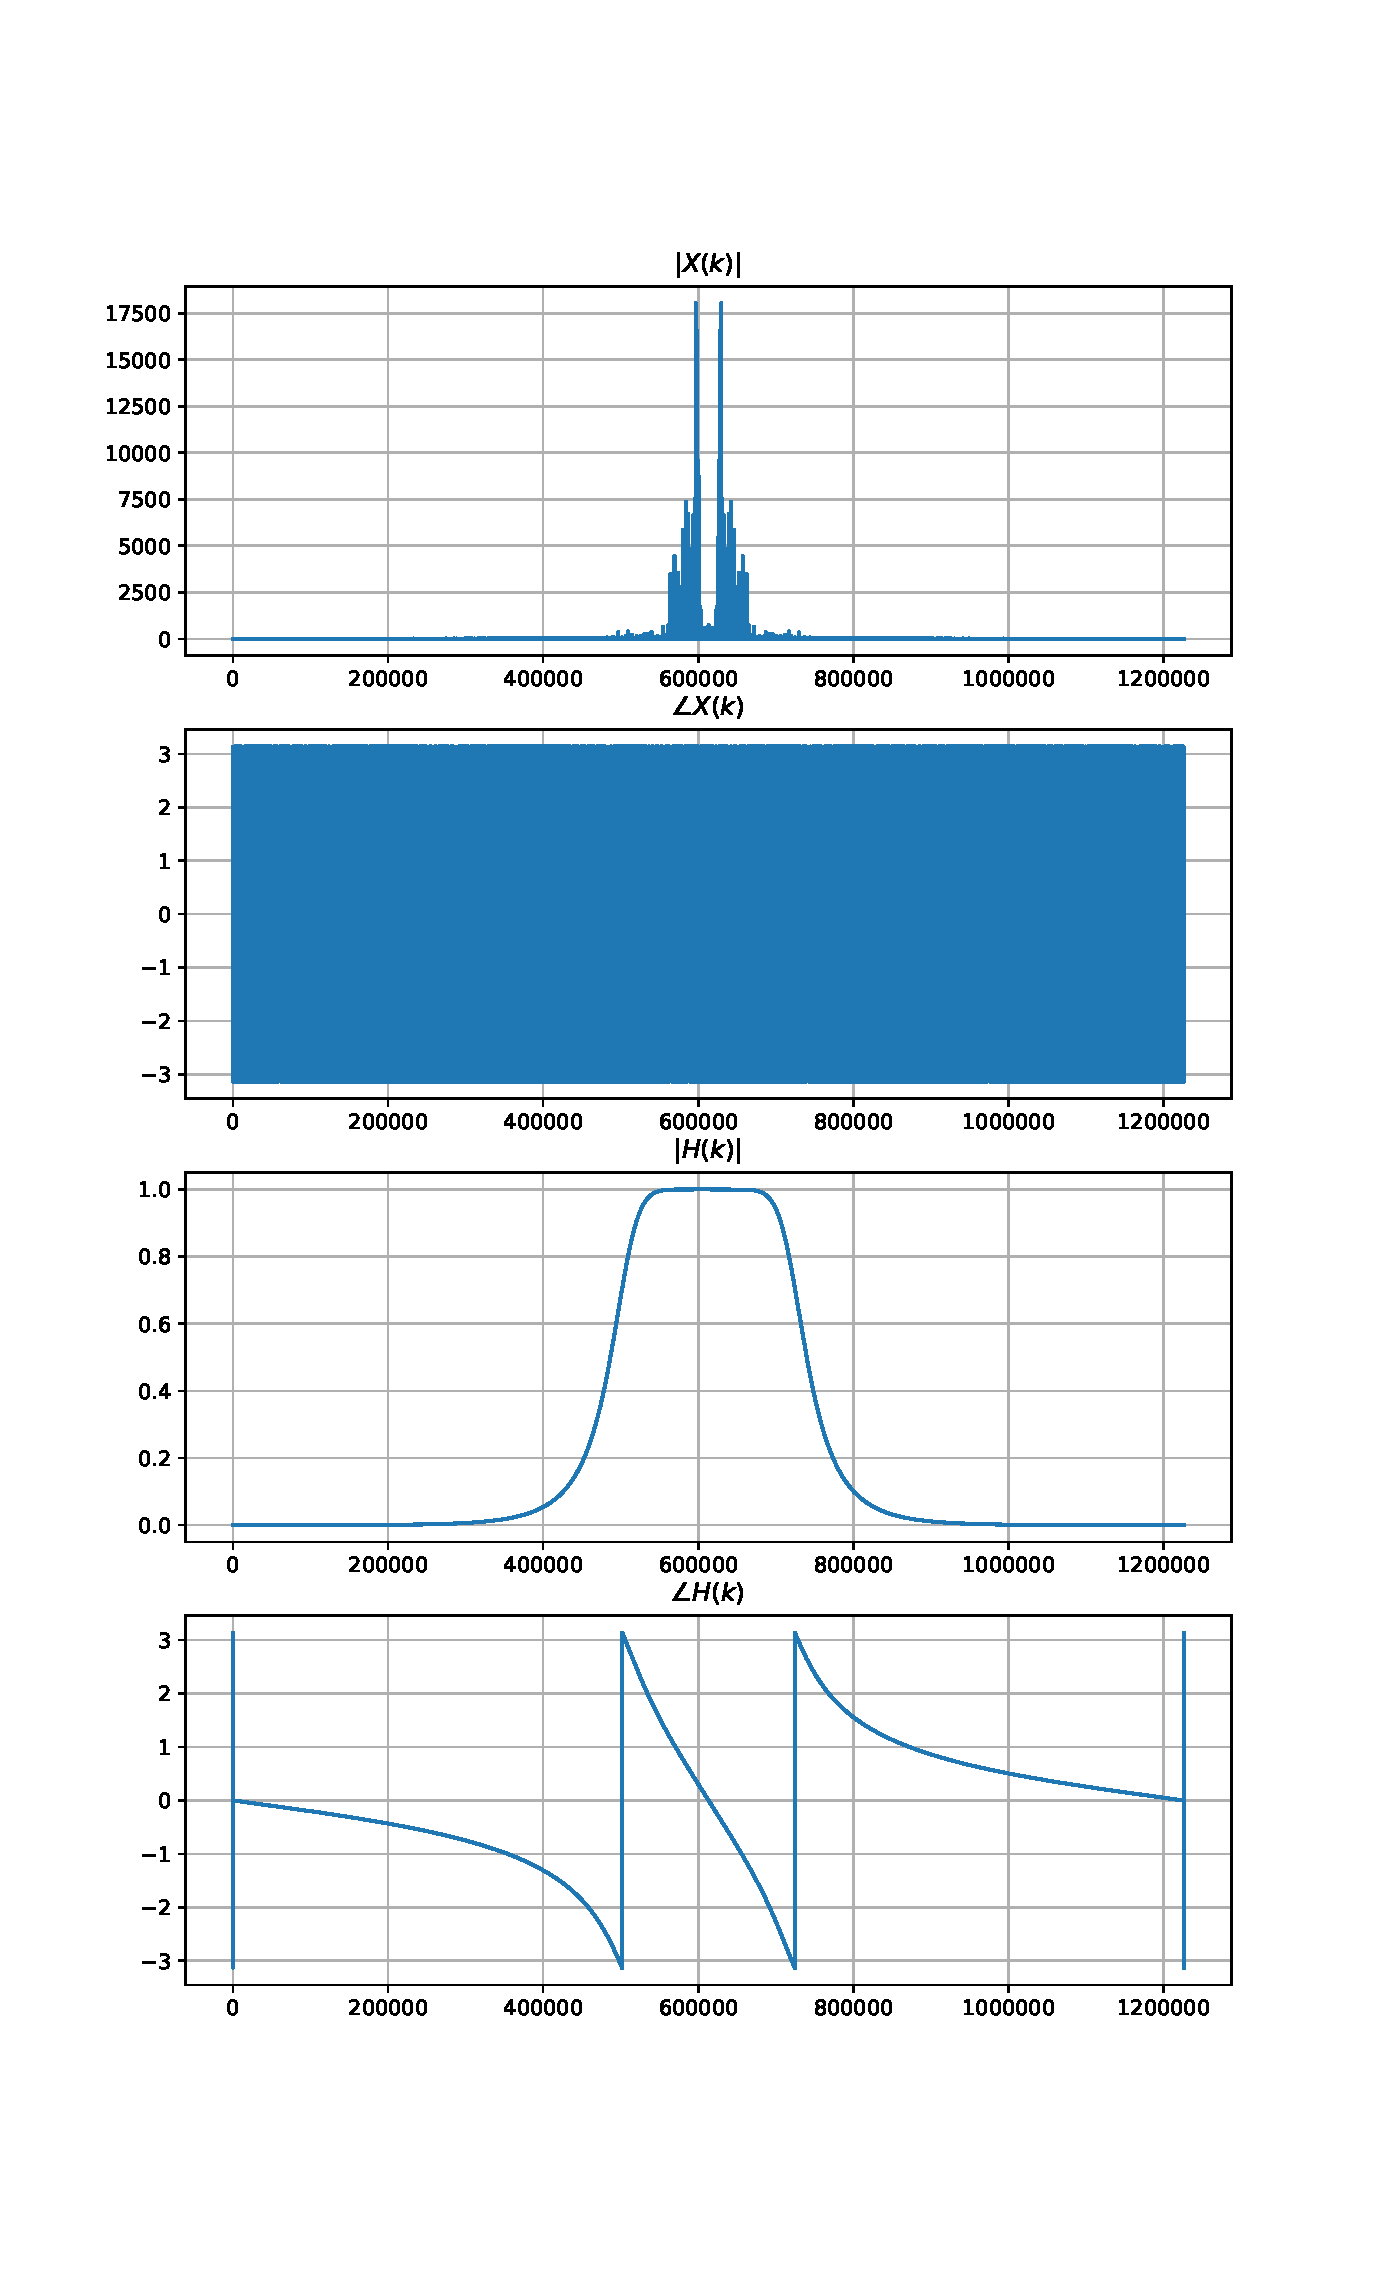
\includegraphics[width=\columnwidth]{./figs/xhfft}
\caption{$X(k)$ and $H(k)$}
\label{fig:xhfft}
\end{figure}

\item Compute
\begin{equation}
Y(k) = X(k)H(k)
\end{equation}
and using this find 
\begin{equation}
y(n) \triangleq \sum_{k=0}^{N-1} Y(k) e^{j 2 \pi k n / N}, \quad n=0,1, \ldots, N-1
\end{equation}
\\
\solution
The following code plots Fig.\ref{fig:yfft}
\begin{lstlisting}
codes/yfft.py
\end{lstlisting}
\begin{figure}[!ht]
\centering
\includegraphics[width=\columnwidth]{./figs/yfft}
\caption{$y(n)$ from IFFT}
\label{fig:yfft}
\end{figure}

The filtered sound signal from this method is found in
\begin{lstlisting}
codes/Sound_fft.wav
\end{lstlisting}
We can observe from the above plot that it is same as the y(n) observed in Fig.\ref{fig:x_y}
\end{enumerate}


\end{document}

